\documentclass[12pt,addpoints]{repaso}
\grado{3}
\nivel{Secundaria}
\cicloescolar{2023-2024}
\materia{Matemáticas}
\unidad{3}
\title{Practica la Unidad}
\aprendizajes{
    \item Comprende las series y sucesiones cuadraticas y geométricas y sus respectivas formulaciones algebraicas.
    \item Reconoce y aplica los principales productos notables y su interpretación geométrica.
    \item Resuelve problemas mediante la formulación y la solución algebraica de ecuaciones cuadráticas. 
    \item Formula, justifica y usa el teorema de Pitágoras para resolver problemas.
    \item Usa las funciones trigonométricas para resolver problemas geométricos con aplicación en la vida diaria.
    }
\author{Melchor Pinto, J.C.}
\begin{document}
\INFO%
\section*{Sucesiones cuadráticas y geométricas}%
% \subsection*{Sucesión cuadrática}%
\ejemplosboxed[{Escribe los primeros 4 términos de las siguientes sucesiones cuadráticas:

            \begin{multicols}{2}
                \begin{parts}
                    \part {\large $2n^2+5n+2$} \hfill \fillin[$9,20,35,54$][0cm]

                    \begin{solutionbox}{2.5cm}
                        $n=1$ \quad $2(1)^2+5(1)+2=9$ \\
                        $n=2$ \quad $2(2)^2+5(2)+2=20$ \\
                        $n=3$ \quad $2(3)^2+5(3)+2=35$ \\
                        $n=4$ \quad $2(4)^2+5(4)+2=54$
                    \end{solutionbox}

                    \part {\large $n^2+5n$} \hfill \fillin[$6,14,24,36$][0cm]

                    \begin{solutionbox}{2.5cm}
                        $n=1$ \quad $(1)^2+5(1)=6$ \\
                        $n=2$ \quad $(2)^2+5(2)=14$ \\
                        $n=3$ \quad $(3)^2+5(3)=24$ \\
                        $n=4$ \quad $(4)^2+5(4)=36$
                    \end{solutionbox}
                \end{parts}
            \end{multicols}
        }]

\begin{questions}
    \questionboxed[6]{Escribe los primeros 4 términos de las siguientes sucesiones cuadráticas:

        \begin{multicols}{3}
            \begin{parts}
                \part {\large $2n^2$ } \hfill \fillin[$2,8,18,32$][0cm]

                \begin{solutionbox}{2.5cm}
                    $n=1$ \quad $2(1)^2=2$ \\
                    $n=2$ \quad $2(2)^2=8$ \\
                    $n=3$ \quad $2(3)^2=18$ \\
                    $n=4$ \quad $2(4)^2=32$
                \end{solutionbox}

                \part {\large $5n^2+2n$}  \hfill \fillin[$7,24,51,88$][0cm]

                \begin{solutionbox}{2.5cm}
                    $n=1$ \quad $5(1)^2+2(1)=7$ \\
                    $n=2$ \quad $5(2)^2+2(2)=24$ \\
                    $n=3$ \quad $5(3)^2+2(3)=51$ \\
                    $n=4$ \quad $5(4)^2+2(4)=88$
                \end{solutionbox}

                \part {\large $n^2-6n$}  \hfill \fillin[$-5,-8,-9,-8$][0.0cm]

                \begin{solutionbox}{2.5cm}
                    $n=1$ \quad $(1)^2-6(1)=-5$ \\
                    $n=2$ \quad $(2)^2-6(2)=-8$ \\
                    $n=3$ \quad $(3)^2-6(3)=-9$ \\
                    $n=4$ \quad $(4)^2-6(4)=-8$
                \end{solutionbox}
            \end{parts}
        \end{multicols}
    }


    \subsection*{Completando la sucesión cuadrática}

    \ejemplosboxed[{Escribe los términos faltantes de las siguientes sucesiones cuadráticas:

                \begin{multicols}{2}
                    \begin{parts}
                        \part {\large $5,12,21,$ \fillin[32][0.5cm],\fillin[45][0.5cm],\fillin[60][0.5cm], \dots}

                        \begin{solutionbox}{2.5cm}\large
                            \quadraticseries{5}{12}{21}
                        \end{solutionbox}

                        \part {\large $-5,-8,-9,$ \fillin[-8][0.5cm],\fillin[-5][0.5cm],\fillin[0][0.5cm], \dots}

                        \begin{solutionbox}{2.5cm}\large
                            \quadraticseries{-5}{-8}{-9}
                        \end{solutionbox}

                    \end{parts}
                \end{multicols}

            }]

    \questionboxed[3]{Escribe los términos faltantes de las siguientes sucesiones cuadráticas:
        \begin{multicols}{3}
            \begin{parts}
                \part {\large $-9,-6,-1,$ \fillin[][0.5cm],\fillin[][0.5cm],\fillin[][0.5cm], \dots}

                \begin{solutionbox}{2.2cm}
                    \quadraticseries{-9}{-6}{-1}
                \end{solutionbox}

                \part {\large $1,5,11,$ \fillin[][0.5cm],\fillin[][0.5cm],\fillin[][0.5cm], \dots}

                \begin{solutionbox}{2.2cm}
                    \quadraticseries{1}{5}{11}
                \end{solutionbox}

                \part {\large $8,20,36,$ \fillin[][0.5cm],\fillin[][0.5cm],\fillin[][0.5cm], \dots}

                \begin{solutionbox}{2.2cm}
                    \quadraticseries{8}{20}{36}
                \end{solutionbox}
            \end{parts}
        \end{multicols}
    }

    \subsection*{Término general}

    \ejemplosboxed[{Determina el término general de las siguientes sucesiones cuadráticas:

                \begin{multicols}{2}
                    \begin{parts}
                        \part {\large $8,15,24,35,\dots$}

                        \begin{solutionbox}{2cm}
                            % \quadraticseries{8}{15}{24}
                            \fillin[$n^2+4n+3$][0cm]
                        \end{solutionbox}

                        \part {\large $6,9,14,21, \dots$}

                        \begin{solutionbox}{2cm}
                            % \quadraticseries{6}{9}{14}
                            \fillin[$n^2+5$][0cm]
                        \end{solutionbox}
                    \end{parts}
                \end{multicols}
            }]

    \questionboxed[3]{Determina el término general de las siguientes sucesiones cuadráticas:

        \begin{multicols}{3}
            \begin{parts}
                \part {\large $4,10,18,28,\dots$}

                \begin{solutionbox}{2cm}
                    \fillin[$n^2+3n$][0cm]
                \end{solutionbox}

                \part {\large $0,3,8,15,\dots$}

                \begin{solutionbox}{2cm}
                    \fillin[$n^2-1$][0cm]
                \end{solutionbox}

                \part {\large $1,13,33,61,\dots$}

                \begin{solutionbox}{2cm}
                    \fillin[$4n^2-3$][0cm]
                \end{solutionbox}
            \end{parts}
        \end{multicols}
    }

    \subsection*{Sucesión geométrica}

    \ejemplosboxed[{Escribe los primeros 4 términos de las siguientes sucesiones geométricas:
                \begin{multicols}{2}
                    \begin{parts}
                        \part {\large $\large a_{n}=-\left( \dfrac{1}{5}\right)^{n-1}$}

                        \begin{solutionbox}{2cm}
                            \fillin[$-1$][0cm], \fillin[$-\dfrac{1}{5}$][0cm], \fillin[$-\dfrac{1}{25}$][0cm], \fillin[$-\dfrac{1}{125}$][0cm]
                        \end{solutionbox}

                        \part {\large $\large a_{n}=4\left( 2\right)^{n-1}$}

                        \begin{solutionbox}{2cm}
                            \fillin[$4$][0cm], \fillin[$8$][0cm], \fillin[$16$][0cm], \fillin[$32$][0cm]
                        \end{solutionbox}
                    \end{parts}
                \end{multicols}
            }]

    \questionboxed[3]{Escribe los primeros 4 términos de las siguientes sucesiones geométricas:
        \begin{multicols}{3}
            \begin{parts}
                \part {\large $\large a_{n}=\left( -2\right)^{n-1}$}

                \begin{solutionbox}{2cm}
                    \fillin[$1$][0cm], \fillin[$-2$][0cm], \fillin[$4$][0cm], \fillin[$-8$][0cm]
                \end{solutionbox}

                \part {\large $\large a_{n}=\left( 4\right)^{n-1}$}

                \begin{solutionbox}{2cm}
                    \fillin[$1$][0cm], \fillin[$4$][0cm], \fillin[$16$][0cm], \fillin[$64$][0cm]
                \end{solutionbox}

                \part {\large $\large a_{n}=2\left( 5\right)^{n-1}$}

                \begin{solutionbox}{2cm}
                    \fillin[$2$][0cm], \fillin[$10$][0cm], \fillin[$50$][0cm], \fillin[$250$][0cm]
                \end{solutionbox}
            \end{parts}
        \end{multicols}
    }

    \subsection*{Razón de una sucesión geométrica}

    \ejemplosboxed[{Determina la razón de las siguientes sucesiones geométricas:
                \begin{multicols}{2}
                    \begin{parts}
                        \part {\large $3,\frac{3}{4}, \frac{3}{16}, \frac{3}{64},\dots$ \quad r=\fillin[$\frac{1}{4}$][0cm]}

                        \begin{solutionbox}{2cm}

                        \end{solutionbox}

                        \part {\large $3,\frac{6}{5}, \frac{12}{25}, \frac{24}{125},\dots$ \quad r=\fillin[$\frac{2}{5}$][0cm]}

                        \begin{solutionbox}{2cm}
                        \end{solutionbox}
                    \end{parts}
                \end{multicols}
            }]

    \questionboxed[3]{Determina la razón de las siguientes sucesiones geométricas:
        \begin{multicols}{3}
            \begin{parts}
                \part {\large $10,4,\frac{8}{5}, \frac{16}{25},\dots$ \quad r=\fillin[$\frac{2}{5}$][0cm]}

                \begin{solutionbox}{2cm}
                \end{solutionbox}

                \part {\large $24, -12, 6, -3, \frac{3}{2}, \dots$ \quad r=\fillin[$\frac{1}{2}$][0cm]}

                \begin{solutionbox}{2cm}
                \end{solutionbox}

                \part {\large $6, 9, \frac{27}{2}, \frac{81}{4}$ \quad r=\fillin[$\frac{3}{2}$][0cm]}

                \begin{solutionbox}{2cm}
                \end{solutionbox}
            \end{parts}
        \end{multicols}
    }

    \newpage
    \section*{Productos notables}
    \subsection*{Binomios conjugados}

    \ejemplosboxed[{Desarrolla los siguientes productos notables:
                \begin{multicols}{2}
                    \begin{parts}
                        \part $(x-15)(x+15)=$ \fillin[$x^2-225$][0cm]

                        \part $(9x-1)(9x+1)=$ \fillin[$81x^2-1$][0cm]

                    \end{parts}
                \end{multicols}
            }]

    \questionboxed[3]{ Desarrolla los siguientes productos notables:
        \begin{multicols}{3}
            \begin{parts}
                \part $(x+7)(x-7)=$ \fillin[$x^2-49$][0cm]

                \part $(x-12y)(x+12y)=$ \fillin[$x^2-144y^2$][0cm]

                \part $(10x-9y)(10x+9y)=$ \fillin[$100x^2-81y^2$][0cm]
            \end{parts}
        \end{multicols}
    }

    \subsection*{Binomios con término común}

    \ejemplosboxed[{Desarrolla los siguientes productos notables:
                \begin{multicols}{2}
                    \begin{parts}
                        \part $(x-5)(x-6)=$ \fillin[$x^2-11x+30$][0cm]
                        \part $(x+4)(x+6)=$ \fillin[$x^2+10x+24$][0cm]
                    \end{parts}
                \end{multicols}
            }]

    \questionboxed[3]{Desarrolla los siguientes productos notables:
        \begin{multicols}{3}
            \begin{parts}
                \part $(x-2)(x+6)=$ \fillin[$x^2+4x-12$][0cm]
                \part $(x+6)(x-10)=$ \fillin[$x^2-4x-60$][0cm]
                \part $(x-9)(x-2)=$ \fillin[$x^2-11x+18$][0cm]
            \end{parts}
        \end{multicols}
    }

    \subsection*{Binomio al cuadrado}

    \ejemplosboxed[{Desarrolla los siguientes binomios al cuadrado:
                \begin{multicols}{2}
                    \begin{parts}
                        \part $(x-7y)^2=$ \fillin[$x^2-14xy+49y^2$][0cm]
                        \part $(x+3)^2=$ \fillin[$x^2+6x+9$][0cm]
                    \end{parts}
                \end{multicols}
            }]

    \questionboxed[3]{Desarrolla los siguientes binomios al cuadrado:
        \begin{multicols}{3}
            \begin{parts}
                \part $(x+7y)^2=$ \fillin[$x^2+14xy+49y^2$][0cm]
                \part $(x-9)^2=$ \fillin[$x^2-18x+81$][0cm]
                \part $(6x+5y)^2=$ \fillin[$ 36x^2+60xy+25y^2$][0cm]
            \end{parts}
        \end{multicols}
    }

    \subsection*{Binomios de la forma (mx+a)(nx+b)}

    \ejemplosboxed[{Desarrolla los siguientes productos notables:
                \begin{multicols}{2}
                    \begin{parts}
                        \part $(4x-3)(2x+9)=$ \fillin[$8x^2+30x-27$][0cm]
                        \part $(3x-5)(3x+6)=$ \fillin[$9x^2+3x-30$][0cm]
                    \end{parts}
                \end{multicols}
            }]

    \questionboxed[3]{Desarrolla los siguientes productos notables:

        \begin{multicols}{3}
            \begin{parts}
                \part $(3x-3)(2x-8)=$ \fillin[$6x^2-30x+24$][0cm]
                \part $(4x-1)(3x+2)=$ \fillin[$12x^2+5x-2$][0cm]
                \part $(3x-3)(2x-8)=$ \fillin[$8x^2+30x-27$][0cm]
            \end{parts}
        \end{multicols}
    }

    \subsection*{Binomio al cubo}

    \ejemplosboxed[{Desarrolla los siguientes binomios al cubo:

                \begin{multicols}{2}
                    \begin{parts}
                        \part $(5x-2y)^3=$ \fillin[$125x^3-150x^2y+60xy^2-8y^3$][0cm]
                        \part $(x-4)^3=$ \fillin[$x^3-12x^2+48x-64$][0cm]
                    \end{parts}
                \end{multicols}
            }]

    \questionboxed[3]{Desarrolla los siguientes binomios al cubo:

        \begin{multicols}{3}
            \begin{parts}
                \part $(x-3)^3=$ \fillin[$x^3-9x^2+27x-27$][0cm]
                \part $(2x+5)^3=$ \fillin[$8x^3+60x^2+150x+125$][0cm]
                \part $(3x-4)^3=$ \fillin[$27x^3-108x^2+144x-64$][0cm]
            \end{parts}
        \end{multicols}
    }

    \section*{Ecuaciones cuadráticas}
    % \subsection*{Clasificación de ecuaciones cuadráticas}
    % \ejemplosboxed[{
    %             \begin{multicols}{2}
    %                 \begin{parts}
    %                     \part  \fillin[][0.5cm]
    %                     \begin{solutionbox}{2cm}
    %                     \end{solutionbox}
    %                     \part \fillin[][0.5cm]
    %                     \begin{solutionbox}{2cm}
    %                     \end{solutionbox}
    %                 \end{parts}
    %             \end{multicols}
    %         }]

    % \questionboxed[3]{
    %     \begin{multicols}{3}
    %         \begin{parts}
    %             \part
    %             \begin{solutionbox}{2cm}
    %             \end{solutionbox}
    %             \part
    %             \begin{solutionbox}{2cm}
    %             \end{solutionbox}
    %             \part
    %             \begin{solutionbox}{2cm}
    %             \end{solutionbox}
    %         \end{parts}
    %     \end{multicols}
    % }

    \subsection*{Discriminante}

    \ejemplosboxed[{Calcula el discriminante y el número de soluciones que tienen cada una de las siguientes equaciones cuadráticas:
                \begin{multicols}{2}
                    \begin{parts}
                        \part $25x^2-10x+1$ \qquad d=\fillin[$0$][0cm], Soluciones: \fillin[$1$][0cm]

                        \begin{solutionbox}{3cm}\small
                            \begin{align*}
                                d & = b^2-4ac          \\
                                d & = (-10)^2-4(25)(1) \\
                                d & = 100-100          \\
                                d & = 0
                            \end{align*}
                        \end{solutionbox}

                        \part $3x^2+8x-9$ \qquad d=\fillin[$172$][0cm], Soluciones: \fillin[$2$][0cm]

                        \begin{solutionbox}{3cm}\small
                            \begin{align*}
                                d & = b^2-4ac        \\
                                d & = (8)^2-4(3)(-9) \\
                                d & = 64+108         \\
                                d & = 172
                            \end{align*}
                        \end{solutionbox}
                    \end{parts}
                \end{multicols}
            }]

    \questionboxed[3]{Calcula el discriminante y el número de soluciones que tienen cada una de las siguientes equaciones cuadráticas:
        \begin{multicols}{3}
            \begin{parts}
                \part $x^2+14x+49$ \qquad Soluciones: \fillin[$1$][0cm]

                \begin{solutionbox}{3cm}
                    d=\fillin[$0$][0cm]
                \end{solutionbox}

                \part $x^2-5x$ \qquad  Soluciones: \fillin[$2$][0cm]

                \begin{solutionbox}{3cm}
                    d=\fillin[$25$][0cm]
                \end{solutionbox}

                \part $3x^2+7x+13$ \qquad Soluciones: \fillin[$0$][0cm]

                \begin{solutionbox}{3cm}
                    d=\fillin[$ -107$][0cm]
                \end{solutionbox}
            \end{parts}
        \end{multicols}
    }

    \subsection*{Ecuaciones cuadráticas incompletas}

    \ejemplosboxed[{Resuelve las siguientes ecuaciones cuadráticas:

                \begin{multicols}{2}
                    \begin{parts}
                        \part $4x^2-7x=0$

                        \begin{solutionbox}{3cm}
                            \begin{align*}
                                0          & =	      4x^2-7x                    \\
                                0          & =		 x(4x -7)                       \\
                                \therefore & x_1 =0 \text{ y } x_2 =\frac{7}{4}
                            \end{align*}
                            % $x_1=0,x_2=\dfrac{7}{4}$
                        \end{solutionbox}

                        \part $3x^2-4x=0$

                        \begin{solutionbox}{3cm}
                            \begin{align*}
                                0          & =	      3x^2-4x                    \\
                                0          & =		 x(3x -4)                       \\
                                \therefore & x_1 =0 \text{ y } x_2 =\frac{4}{3}
                            \end{align*}
                            % $x_1=0,x_2=\dfrac{4}{3}$
                        \end{solutionbox}
                    \end{parts}
                \end{multicols}
            }]

    \questionboxed[6]{Resuelve las siguientes ecuaciones cuadráticas:

        \begin{multicols}{3}
            \begin{parts}
                \part $x^2+9x=0$

                \begin{solutionbox}{4cm}
                    \begin{align*}
                        0          & =	      x^2+9x            \\
                        0          & =		 x(x+9)                \\
                        \therefore & x_1 =-9 \text{ y } x_2 =0
                    \end{align*}
                    % $x_1=-9,x_2=0$
                \end{solutionbox}

                \columnbreak%

                \part $x^2-49=0$

                \begin{solutionbox}{4cm}\small
                    \begin{align*}
                        0          & =	      x^2-49            \\
                        49         & =		 x^2                   \\
                        \sqrt{49}  & =		 x                     \\
                        \pm 7      & = x                       \\
                        \therefore & x_1 =-7 \text{ y } x_2 =7
                    \end{align*}
                    % $x_1=-7,x_2=7$
                \end{solutionbox}

                \columnbreak%

                \part $x^2+4x=0$

                \begin{solutionbox}{4cm}
                    \begin{align*}
                        0          & =	      x^2+4x            \\
                        0          & =		 x(x+4)                \\
                        \therefore & x_1 =-4 \text{ y } x_2 =0
                    \end{align*}
                    % $x_1=-4,x_2=0$
                \end{solutionbox}
            \end{parts}
        \end{multicols}
    }

    \subsection*{Ecuaciones cuadráticas completas}

    \ejemplosboxed[{Resuelve las siguientes ecuaciones cuadráticas:

                \begin{multicols}{2}
                    \begin{parts}
                        \part $x^2-13x+30=0$

                        \begin{solutionbox}{5cm}
                            \begin{align*}
                                x_{1,\:2} & =\frac{-\left(-13\right)\pm \sqrt{\left(-13\right)^2-4\cdot \:1\cdot \:30}}{2\cdot \:1} \\
                                x_{1,\:2} & =\frac{-\left(-13\right)\pm \:7}{2\cdot \:1}                                            \\
                                x_1       & =\frac{-\left(-13\right)+7}{2\cdot \:1}=10                                              \\
                                x_2       & =\frac{-\left(-13\right)-7}{2\cdot \:1}=3
                            \end{align*}
                            % $x_1=3,x_2=10$
                        \end{solutionbox}

                        \part $x^2+2x-63=0$

                        \begin{solutionbox}{5cm}
                            \begin{align*}
                                x_{1,\:2} & =\frac{-2\pm \sqrt{2^2-4\cdot \:1\cdot \left(-63\right)}}{2\cdot \:1} \\
                                x_{1,\:2} & =\frac{-2\pm \:16}{2\cdot \:1}                                        \\
                                x_1       & =\frac{-2+16}{2\cdot \:1}=7                                           \\
                                x_2       & =\frac{-2-16}{2\cdot \:1}=-9
                            \end{align*}
                            % $x_1=-9,x_2=7$
                        \end{solutionbox}
                    \end{parts}
                \end{multicols}
            }]

    \questionboxed[6]{Resuelve las siguientes ecuaciones cuadráticas:

        \begin{multicols}{3}
            \begin{parts}
                \part $x^2-3x-40=0$

                \begin{solutionbox}{2cm}
                    $x_1=-5,x_2=8$
                \end{solutionbox}

                \part $x^2-3x-28=0$

                \begin{solutionbox}{2cm}
                    $x_1=-4,x_2=7$
                \end{solutionbox}

                \part $x^2-2x-15=0$

                \begin{solutionbox}{2cm}
                    $x_1=-3,x_2=5$
                \end{solutionbox}

                % \columnbreak%

                \part $2x^2-9x-5=0$

                \begin{solutionbox}{2cm}
                    $x_1=-\dfrac{1}{2},x_2=5$
                \end{solutionbox}

                \part $20x^2+23x+6=0$

                \begin{solutionbox}{2cm}
                    $x_1=-\dfrac{3}{4},x_2=-\dfrac{2}{5}$
                \end{solutionbox}

                \part $4x^2+5x-6=0$

                \begin{solutionbox}{2cm}
                    $x_1=-2,x_2=\dfrac{3}{4}$
                \end{solutionbox}
            \end{parts}
        \end{multicols}
    }


    \section*{Teorema de Pitágoras}
    % \subsection*{Identificación de lados}

    % \ejemplosboxed[{
    %             \begin{multicols}{2}
    %                 \begin{parts}
    %                     \part  \fillin[][0.5cm]
    %                     \begin{solutionbox}{2cm}
    %                     \end{solutionbox}
    %                     \part \fillin[][0.5cm]
    %                     \begin{solutionbox}{2cm}
    %                     \end{solutionbox}
    %                 \end{parts}
    %             \end{multicols}
    %         }]

    % \questionboxed[3]{
    %     \begin{multicols}{3}
    %         \begin{parts}
    %             \part
    %             \begin{solutionbox}{2cm}
    %             \end{solutionbox}
    %             \part
    %             \begin{solutionbox}{2cm}
    %             \end{solutionbox}
    %             \part
    %             \begin{solutionbox}{2cm}
    %             \end{solutionbox}
    %         \end{parts}
    %     \end{multicols}
    % }


    \subsection*{Hallando la hipotenusa y catetos}

    \ejemplosboxed[{En los siguientes triángulos rectángulos, calcula el lado $x$ que falta:
                \begin{multicols}{2}
                    \begin{parts}
                        \part 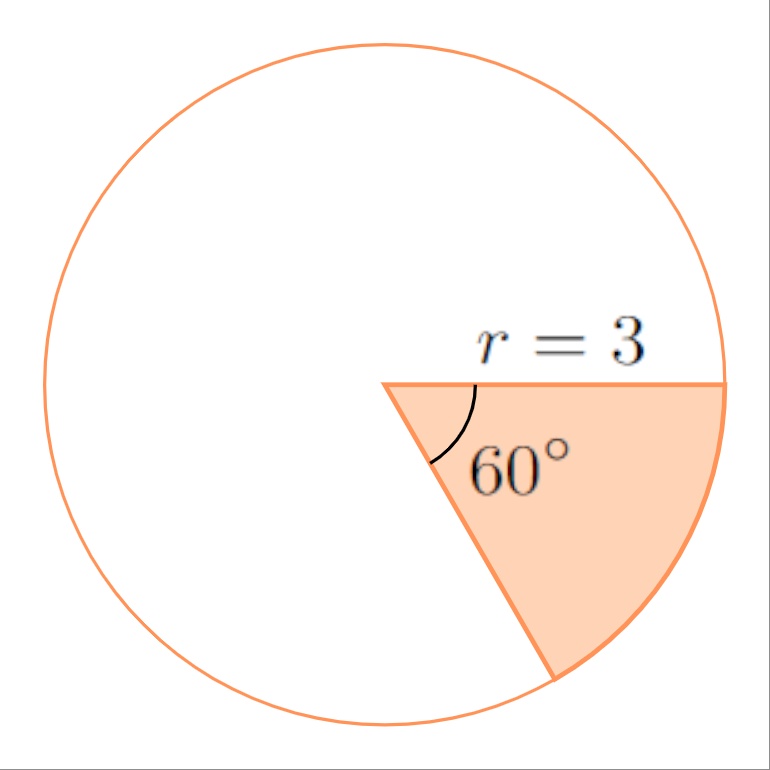
\includegraphics[width=0.6\linewidth]{mex_0061.png} $x=$\fillin[$38.11$][0cm]

                        \begin{solutionbox}{4cm}
                            \begin{align*}
                                c^2                & = a^2 + b^2  \\
                                44^2               & = 22^2 + x^2 \\
                                44^2 - 22^2        & = x^2        \\
                                \sqrt{44^2 - 22^2} & = x          \\
                                38.11              & \simeq x     \\
                            \end{align*}
                        \end{solutionbox}

                        \part 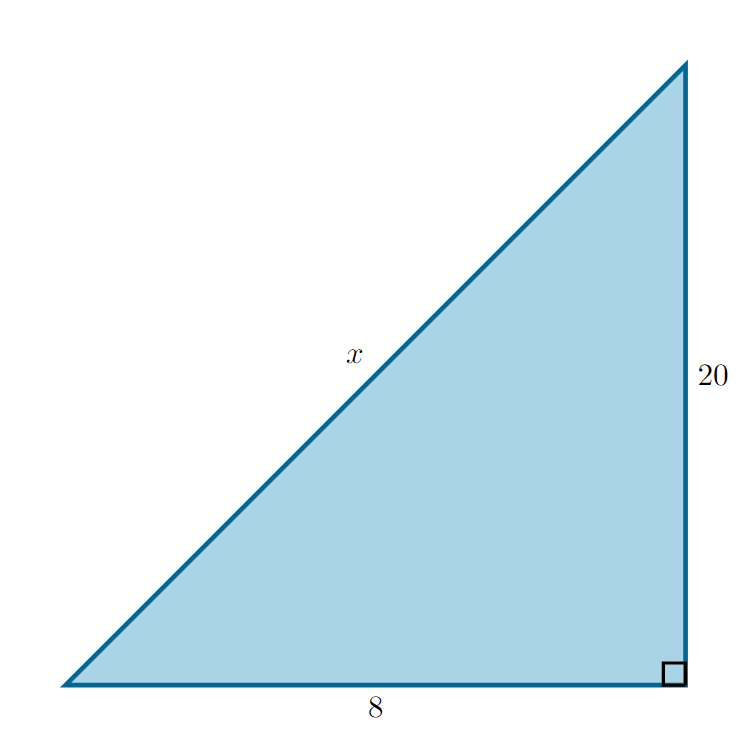
\includegraphics[width=0.6\linewidth]{mex_0057.png} $x=$\fillin[$21.54$][0cm]

                        \begin{solutionbox}{4cm}
                            \begin{align*}
                                c^2 & = a^2 + b^2  \\
                                x^2 & = 8^2 + 20^2 \\
                                x^2 & = 64 + 400   \\
                                x   & = \sqrt{464} \\
                                x   & \simeq 21.54 \\
                            \end{align*}
                        \end{solutionbox}
                    \end{parts}
                \end{multicols}
            }]

    \questionboxed[6]{En los siguientes triángulos rectángulos, calcula el lado $x$ que falta:
        \begin{multicols}{3}
            \begin{parts}
                \part 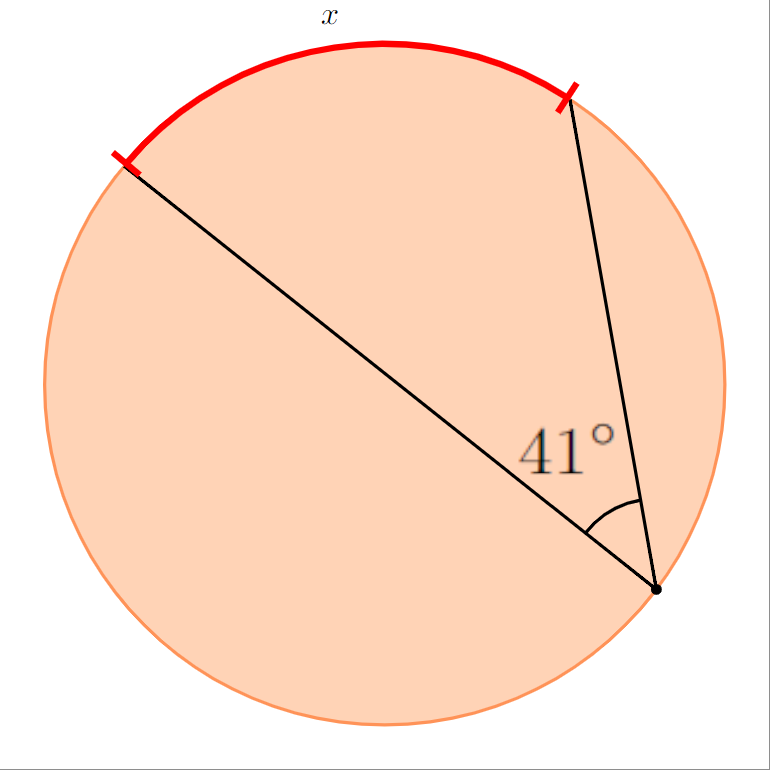
\includegraphics[width=0.9\linewidth]{mex_0056.png} $x=$\fillin[][0cm]

                \begin{solutionbox}{3cm}
                \end{solutionbox}

                \part 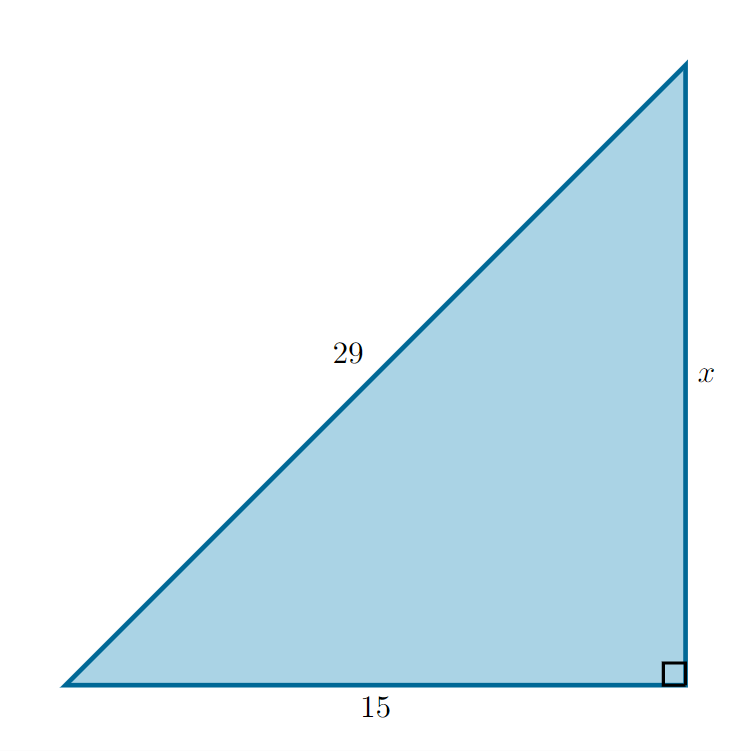
\includegraphics[width=0.9\linewidth]{mex_0064.png} $x=$\fillin[][0cm]

                \begin{solutionbox}{3cm}
                \end{solutionbox}

                \part 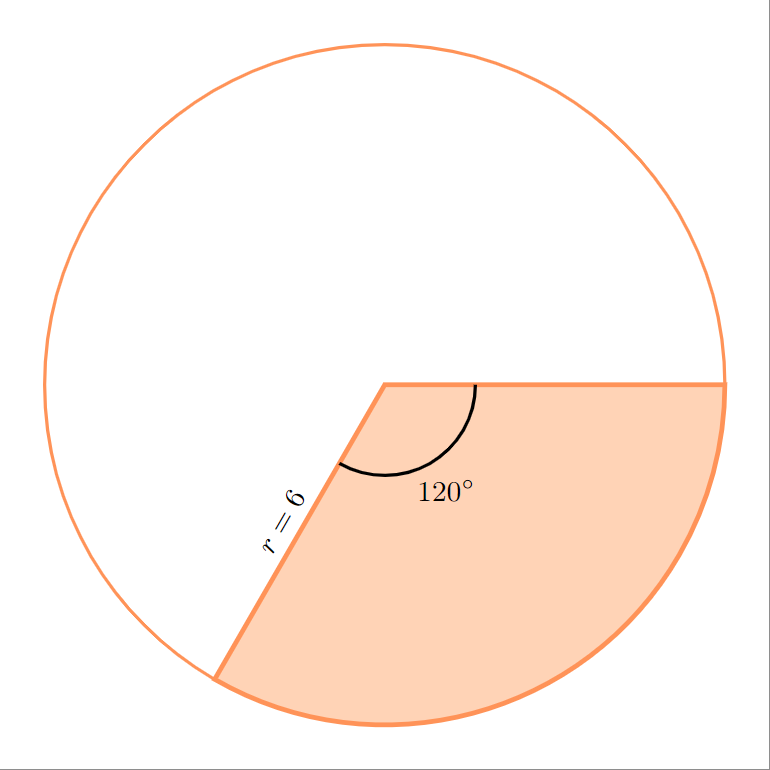
\includegraphics[width=0.9\linewidth]{mex_0062.png} $x=$\fillin[][0cm]

                \begin{solutionbox}{3cm}
                \end{solutionbox}

                \part 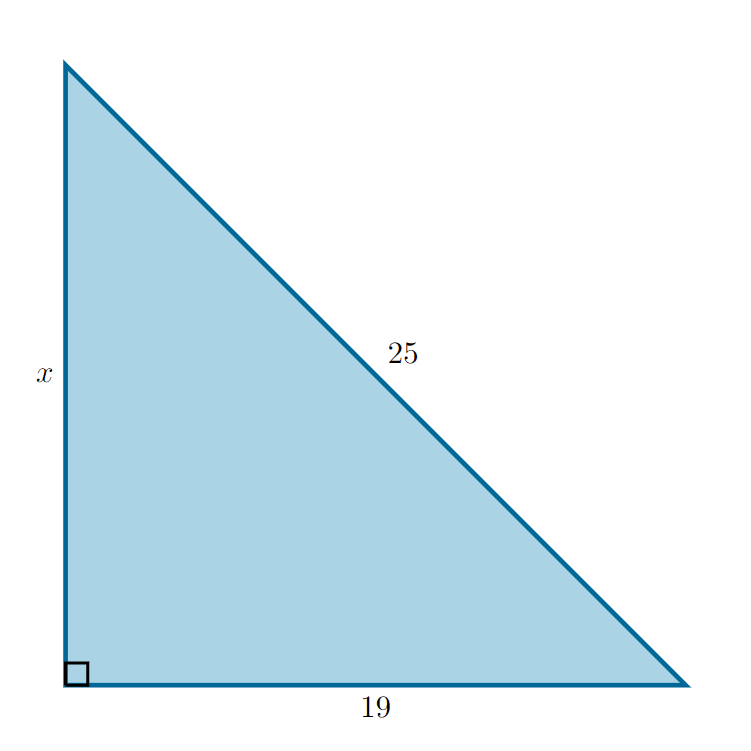
\includegraphics[width=0.9\linewidth]{mex_0065.png} $x=$\fillin[][0cm]

                \begin{solutionbox}{3cm}
                \end{solutionbox}

                \part 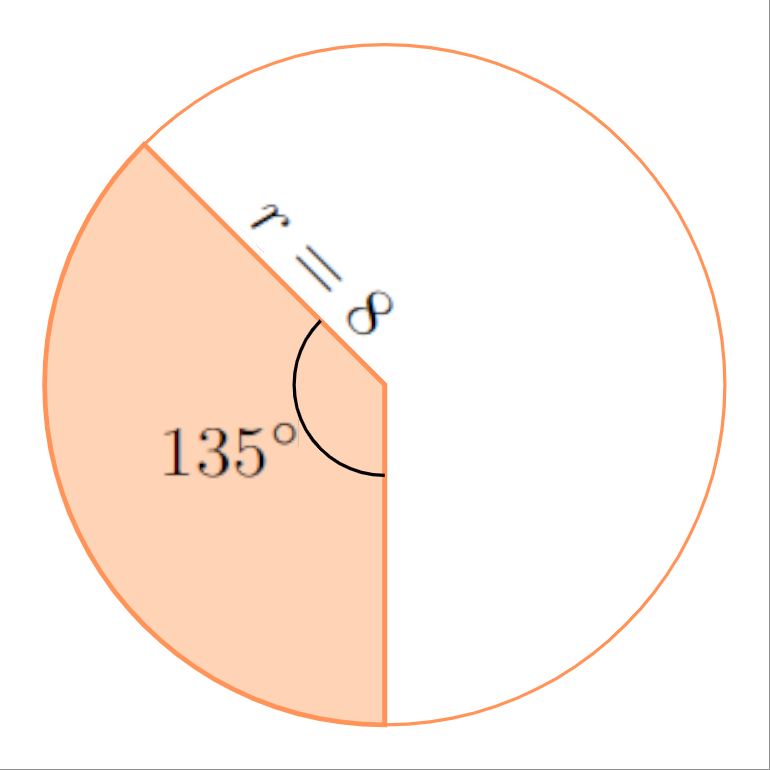
\includegraphics[width=0.9\linewidth]{mex_0063.png} $x=$\fillin[][0cm]

                \begin{solutionbox}{3cm}
                \end{solutionbox}

                \part 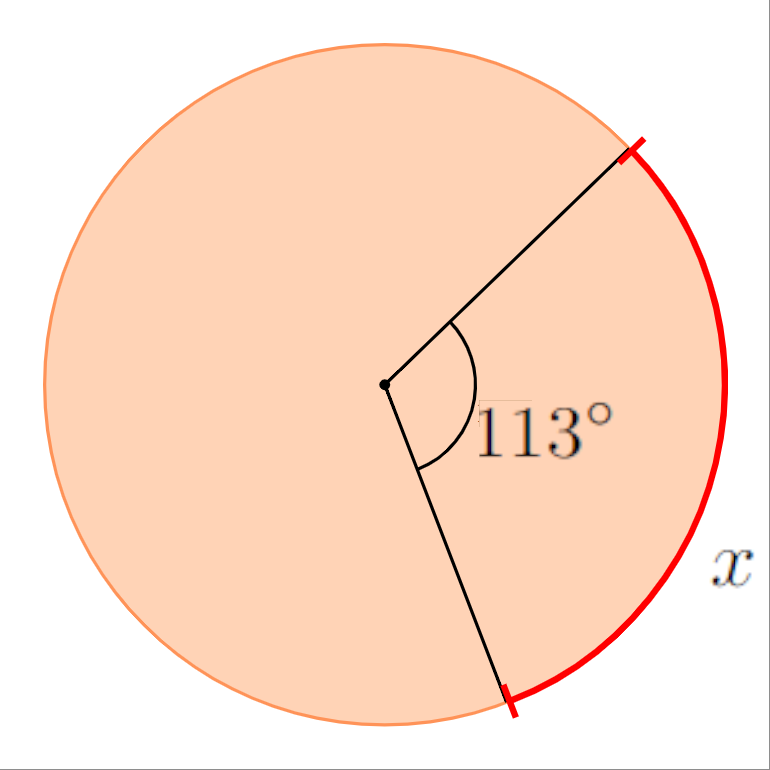
\includegraphics[width=0.9\linewidth]{mex_0055.png} $x=$\fillin[][0cm]

                \begin{solutionbox}{3cm}
                \end{solutionbox}

            \end{parts}
        \end{multicols}
    }

    % \subsection*{Hallando el cateto}

    % \ejemplosboxed[{
    %             \begin{multicols}{2}
    %                 \begin{parts}
    %                     \part  \fillin[][0.5cm]
    %                     \begin{solutionbox}{2cm}
    %                     \end{solutionbox}
    %                     \part \fillin[][0.5cm]
    %                     \begin{solutionbox}{2cm}
    %                     \end{solutionbox}
    %                 \end{parts}
    %             \end{multicols}
    %         }]

    % \questionboxed[6]{
    %     \begin{multicols}{3}
    %         \begin{parts}
    %             \part
    %             \begin{solutionbox}{2cm}
    %             \end{solutionbox}
    %             \part
    %             \begin{solutionbox}{2cm}
    %             \end{solutionbox}
    %             \part
    %             \begin{solutionbox}{2cm}
    %             \end{solutionbox}
    %         \end{parts}
    %     \end{multicols}
    % }

    \subsection*{Áreas y perímetros}

    \ejemplosboxed[{Encuentra el perímetro y el área de las siguientes figuras:

                \begin{multicols}{2}
                    \begin{parts}
                        \part  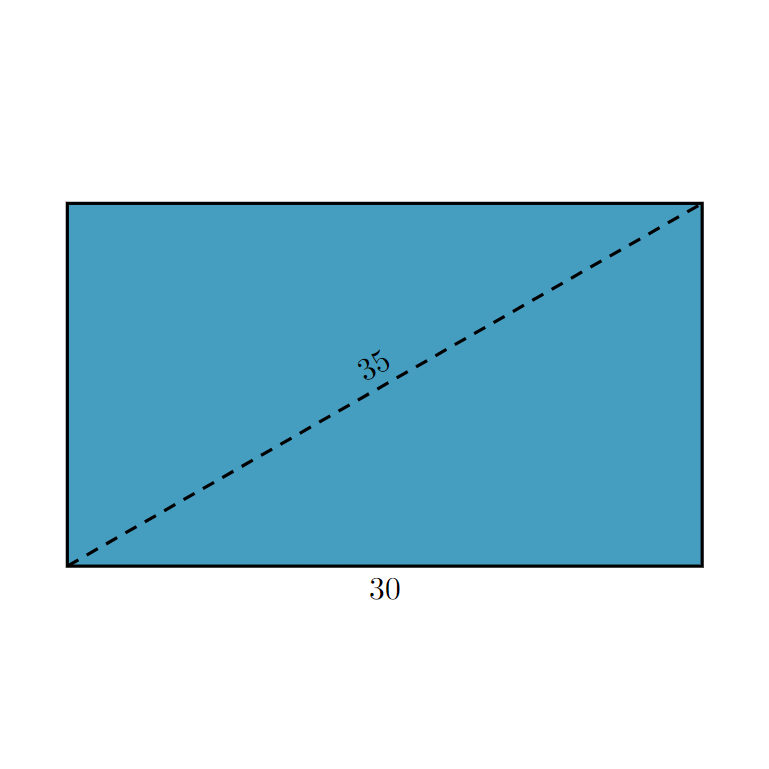
\includegraphics[width=0.8\linewidth]{mex_0066.png} $x=$\fillin[][0cm]

                        \begin{solutionbox}{3cm}
                        \end{solutionbox}

                        \part 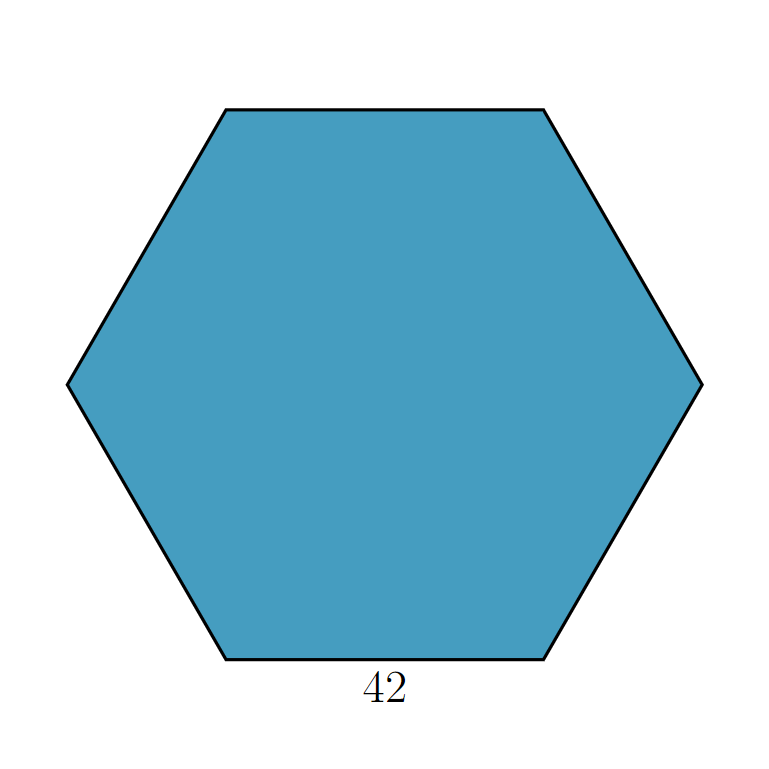
\includegraphics[width=0.8\linewidth]{mex_0067.png} $x=$\fillin[][0cm]

                        \begin{solutionbox}{3cm}
                        \end{solutionbox}
                    \end{parts}
                \end{multicols}
            }]

    \questionboxed[12]{Encuentra el perímetro y el área de las siguientes figuras:

        \begin{multicols}{3}
            \begin{parts}
                \part  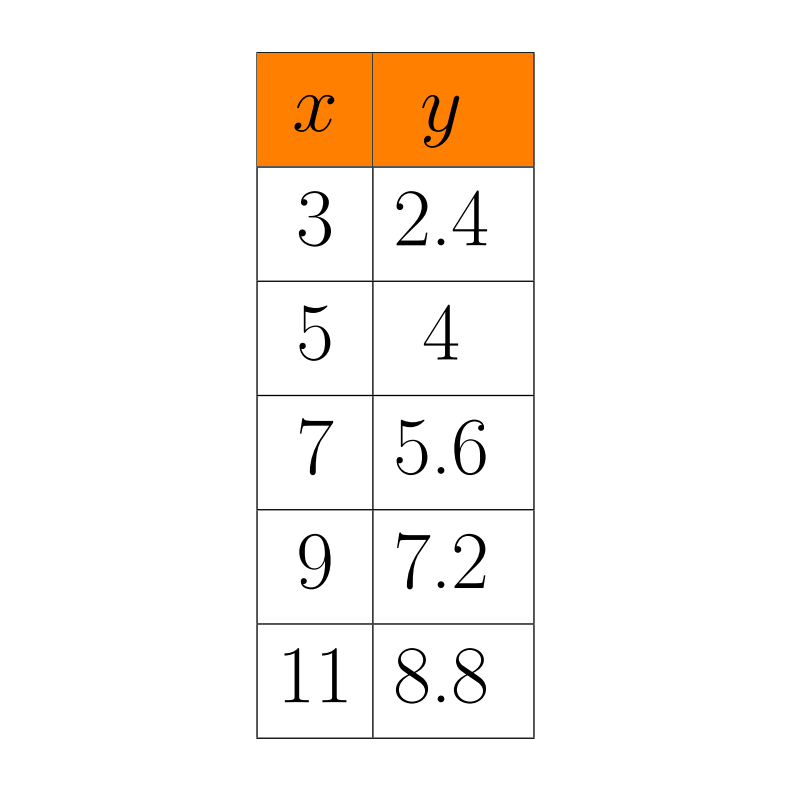
\includegraphics[width=0.9\linewidth]{mex_0068.png}

                \begin{solutionbox}{3cm}
                    Perímetro:

                    Área:

                \end{solutionbox}

                \part 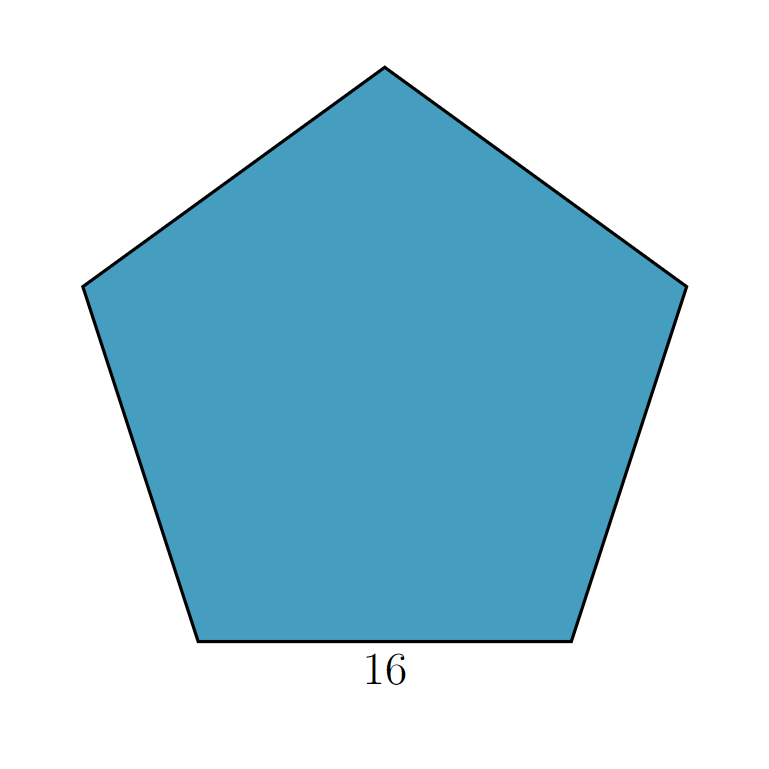
\includegraphics[width=0.9\linewidth]{mex_0069.png}

                \begin{solutionbox}{3cm}
                    Perímetro:

                    Área:
                \end{solutionbox}

                \part  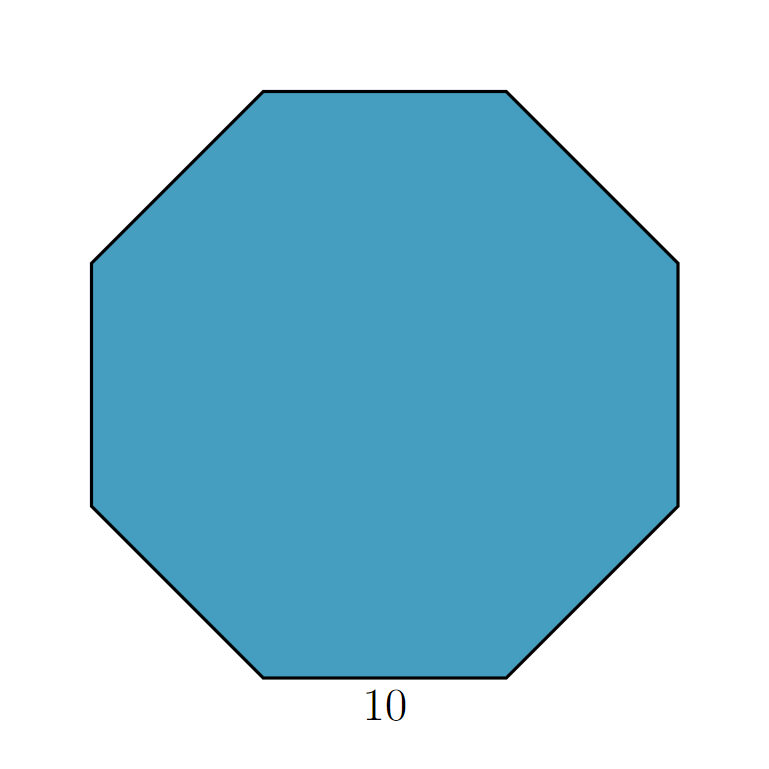
\includegraphics[width=0.9\linewidth]{mex_0070.png}

                \begin{solutionbox}{3cm}
                    Perímetro:

                    Área:
                \end{solutionbox}


            \end{parts}
        \end{multicols}
    }

    \subsection*{Resolución de problemas}

    \ejemplosboxed[{Resuelve los siguientes problemas:

                \begin{multicols}{2}
                    \begin{parts}
                        \part  Desde la ventana de una torre en la playa se ve un barco a 85 metros, cuando realmente se encuentra a 84 metros de la torre. ¿A qué altura está la ventana?

                        \begin{solutionbox}{2cm}
                            13
                        \end{solutionbox}

                        \part Calcula la altura de un triángulo isósceles cuya base mide 12 cm y sus lados iguales miden 25 cm.

                        \begin{solutionbox}{2cm}
                            24.26
                        \end{solutionbox}
                    \end{parts}
                \end{multicols}
            }]

    \questionboxed[10]{Resuelve los siguientes problemas:
        % \begin{multicols}{3}

        \begin{parts}
            \part En una rampa, un ciclista avanza una distancia real de 85 metros mientras que avanza una distancia horizontal de 78 metros. ¿Cuál es la altura de la rampa?

            \begin{solutionbox}{2cm}
                33.77
            \end{solutionbox}

            \part La altura de una portería de fútbol es de 2.4 metros y la distancia desde el punto de penalti hasta la raya de gol es de 10.8 metros, ¿qué distancia recorre un balón si sale desde el punto de penalti y se estrella en la parte más alta de la portería?

            \begin{solutionbox}{2cm}
                11.06
            \end{solutionbox}

            % \part  Calcula la altura que podemos alcanzar con una escalera de 4 metros de longitud apoyada sobre la pared, si la parte inferior de la escalera está a .80 metros de parte de abajo de la pared.

            % \begin{solutionbox}{2cm}
            %     3.91
            % \end{solutionbox}
        \end{parts}
        % \end{multicols}
    }

    \section*{Trigonometría}
    \subsection*{Identificando lados}

    \ejemplosboxed[{¿Cuál es el cateto opuesto del ángulo A?
                \begin{multicols}{2}
                    \begin{parts}
                        \part $CO=$\fillin[$y$][0cm] 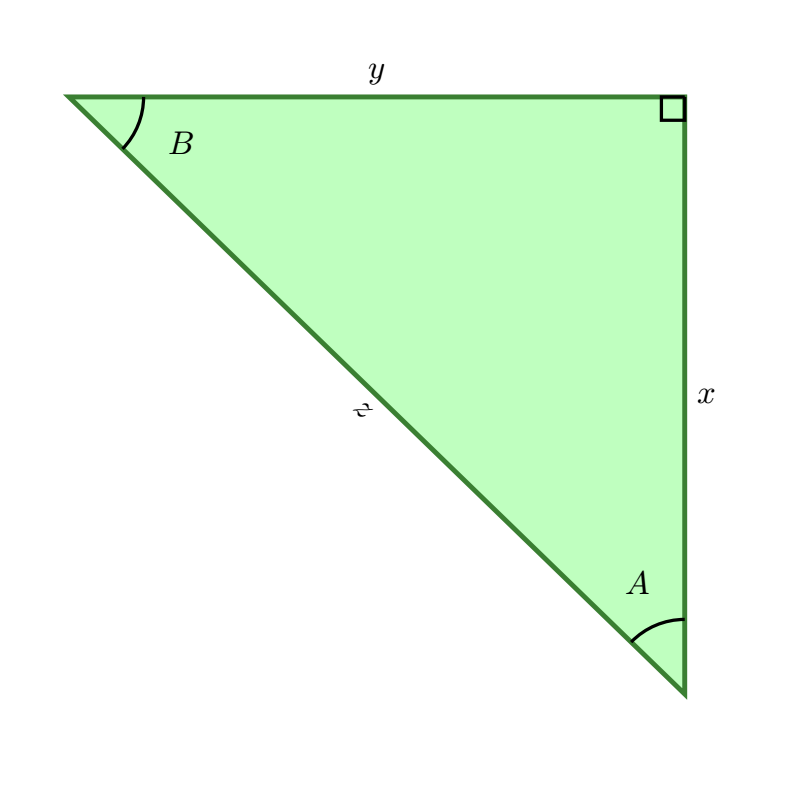
\includegraphics[width=0.8\linewidth]{mex_0075.png}
                        \part $CO=$\fillin[$b$][0cm] 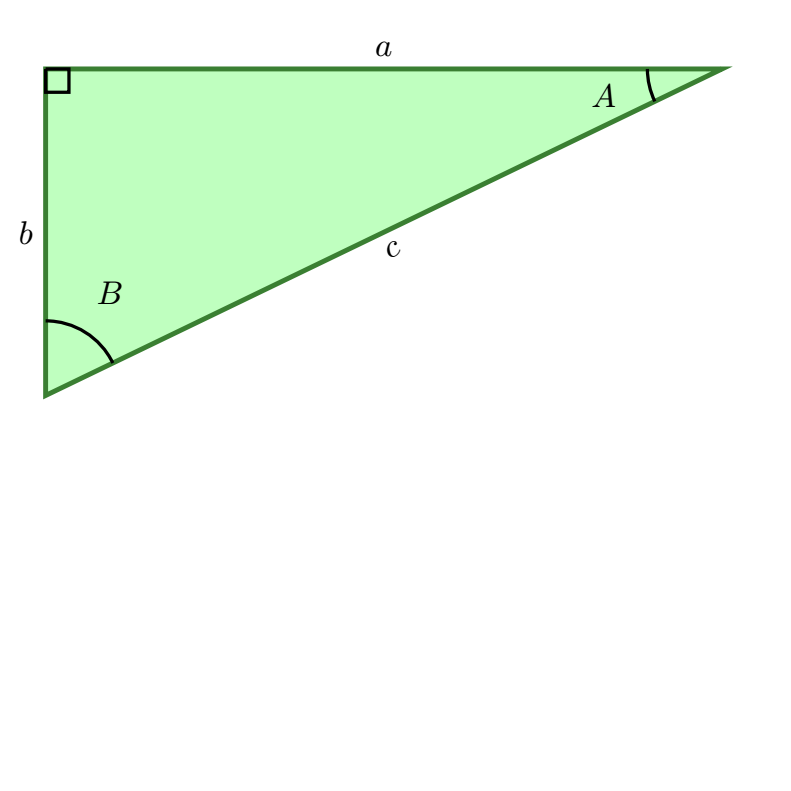
\includegraphics[width=0.65\linewidth]{mex_0072.png}
                    \end{parts}
                \end{multicols}
            }]

    \questionboxed[3]{¿Cuál es el cateto opuesto del ángulo B?

        \begin{multicols}{3}
            \begin{parts}
                \part $CO=$\fillin[$x$][0cm]  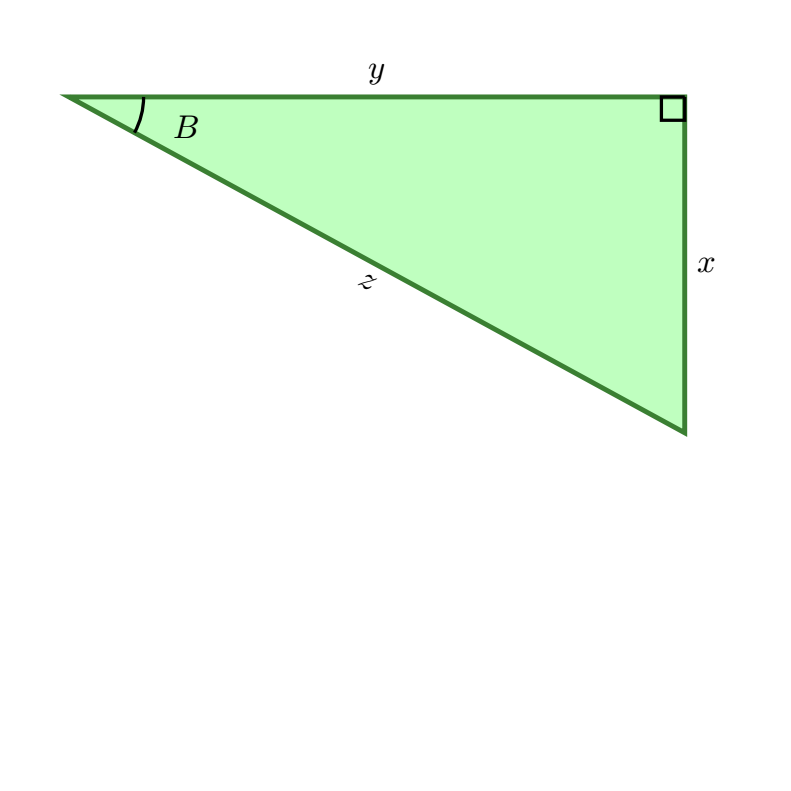
\includegraphics[width=0.95\linewidth]{mex_0078.png}
                \part $CO=$\fillin[$d$][0cm] 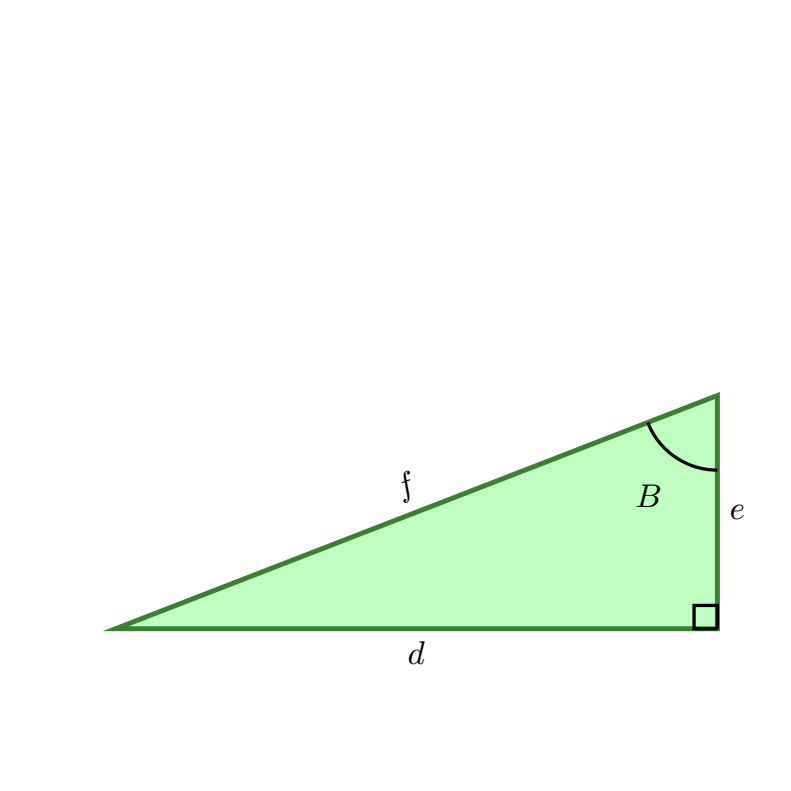
\includegraphics[width=0.95\linewidth]{mex_0079.png}
                \part $CO=$\fillin[$a$][0cm]  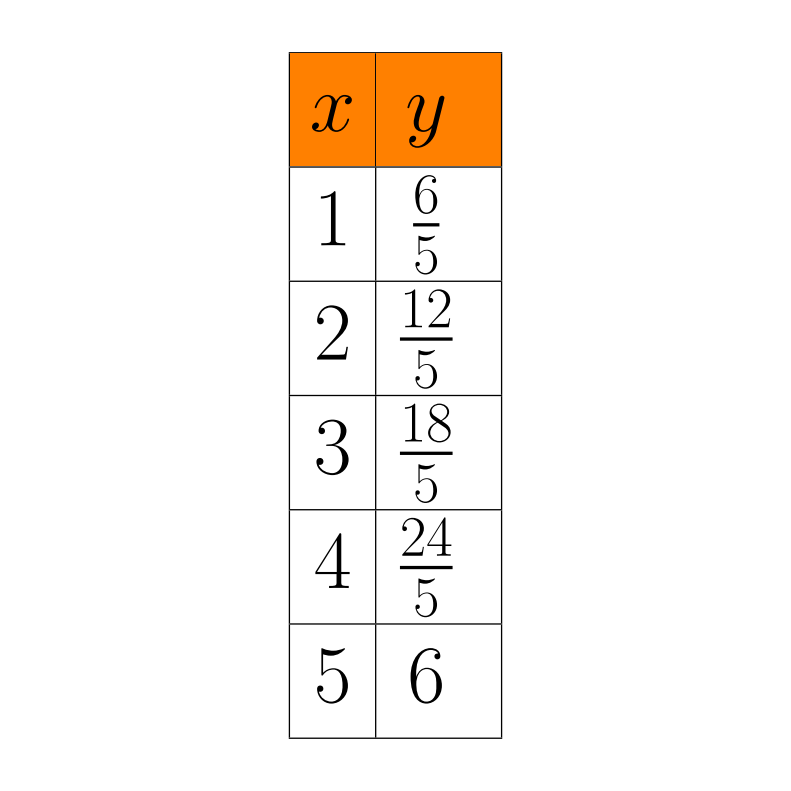
\includegraphics[width=0.9\linewidth]{mex_0076.png}
            \end{parts}
        \end{multicols}
    }
    \questionboxed[3]{¿Cuál es el cateto opuesto del ángulo A?

        \begin{multicols}{3}
            \begin{parts}
                \part $CO=$\fillin[$c$][0cm]  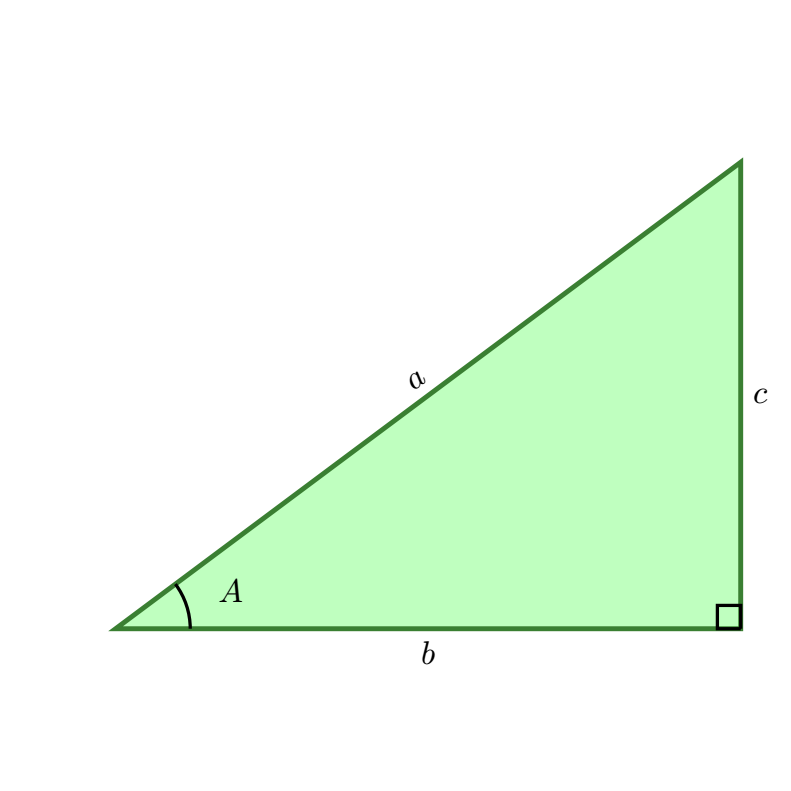
\includegraphics[width=0.95\linewidth]{mex_0071.png}
                \part $CO=$\fillin[$b$][0cm] 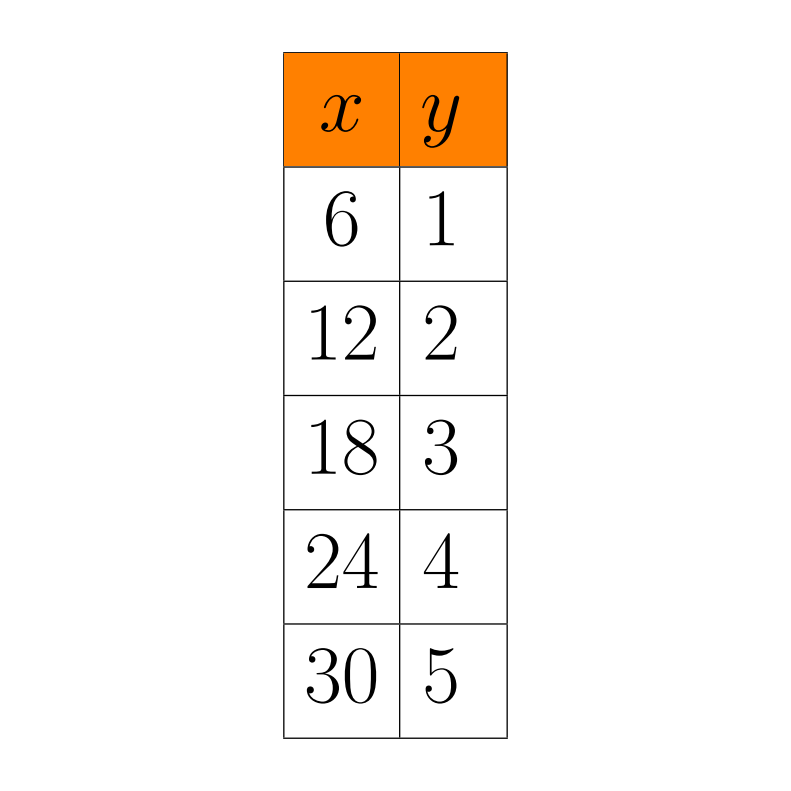
\includegraphics[width=0.95\linewidth]{mex_0074.png}
                \part $CO=$\fillin[$c$][0cm]  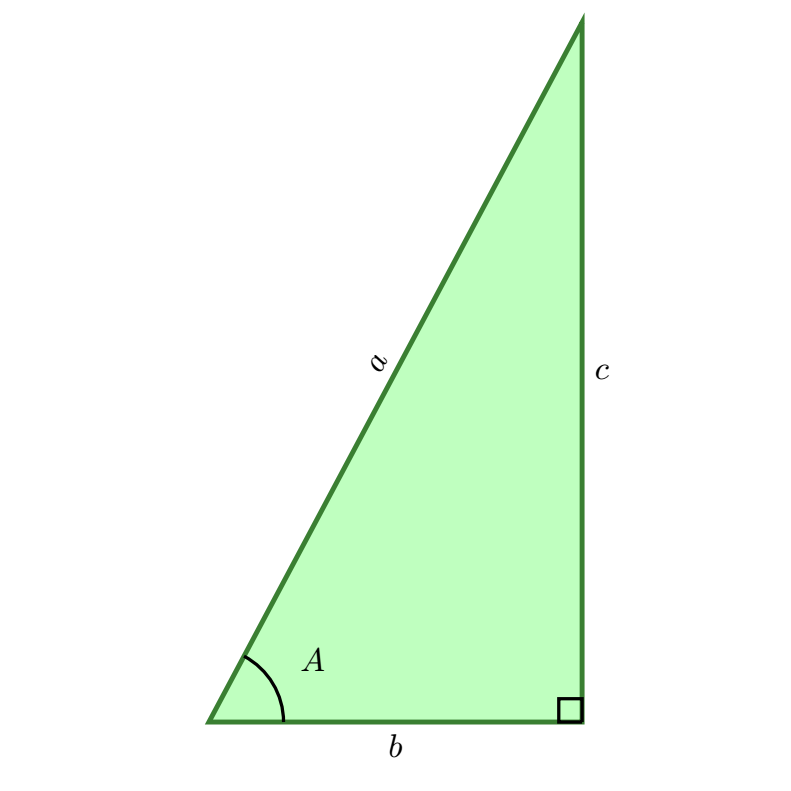
\includegraphics[width=0.9\linewidth]{mex_0073.png}
            \end{parts}
        \end{multicols}
    }


    \subsection*{Identificando funciones}

    \ejemplosboxed[{Con base en las siguientes imágenes, calcula lo que se te pide:

                \begin{multicols}{2}
                    \begin{parts}
                        \part {\Large 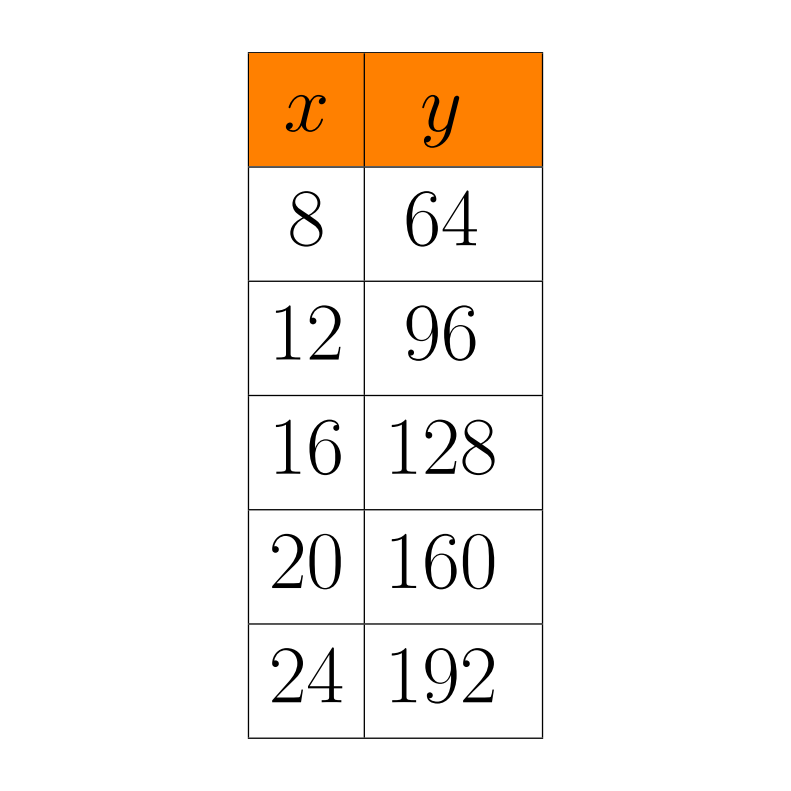
\includegraphics[width=0.75\linewidth]{mex_0081.png} \\ sen($B$)=\fillin[$0.24$][0cm]}
                        \part {\Large 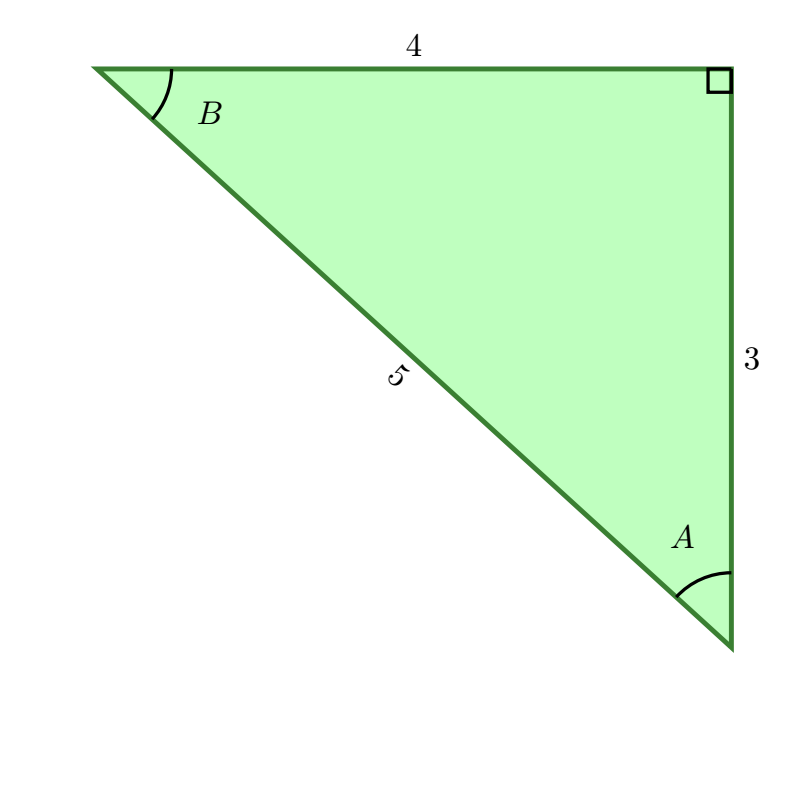
\includegraphics[width=0.75\linewidth]{mex_0082.png} \\ cos($A$)=\fillin[$0.60$][0cm]}
                    \end{parts}
                \end{multicols}
            }]

    \questionboxed[3]{Con base en las siguientes imágenes, calcula lo que se te pide:

        \begin{multicols}{3}
            \begin{parts}
                \part {\large 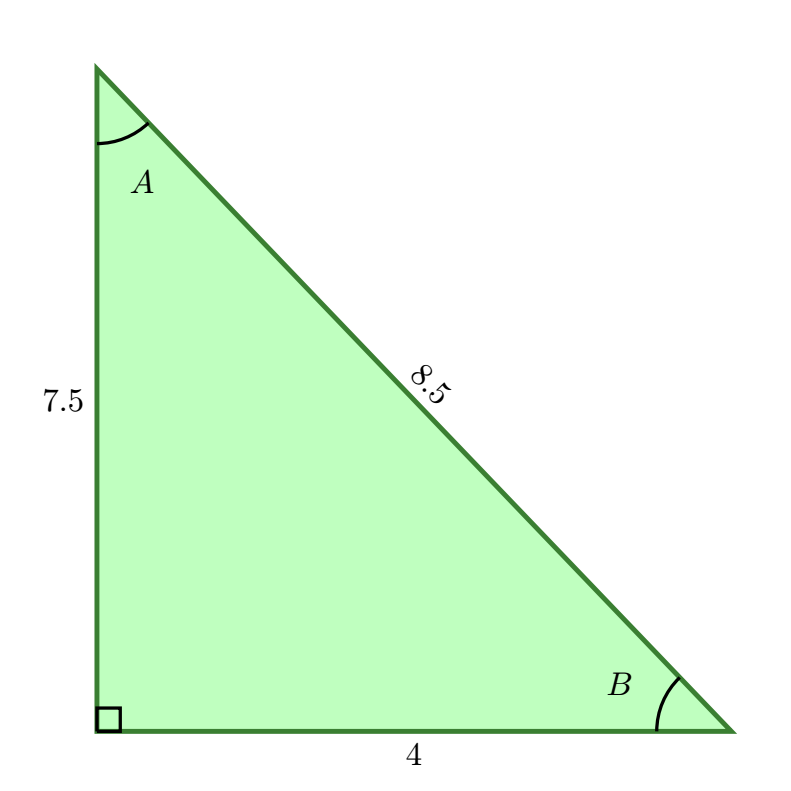
\includegraphics[width=0.9\linewidth]{mex_0088.png} \\ sen($A$)=\fillin[$0.47$][0cm]}
                \part {\large 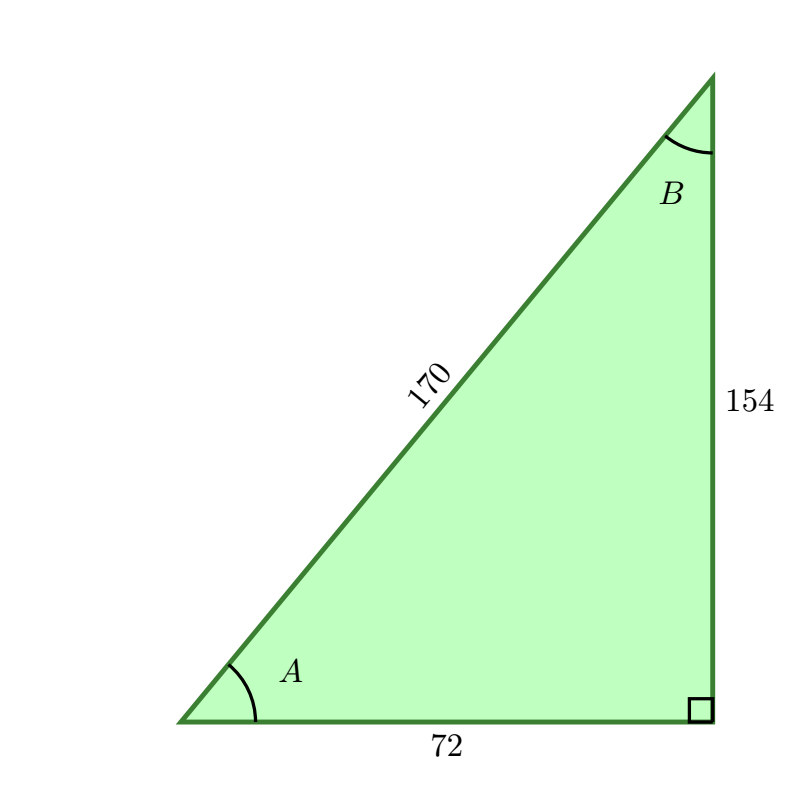
\includegraphics[width=0.9\linewidth]{mex_0085.png} \\ cos($A$)=\fillin[$0.42$][0cm]}
                \part {\large 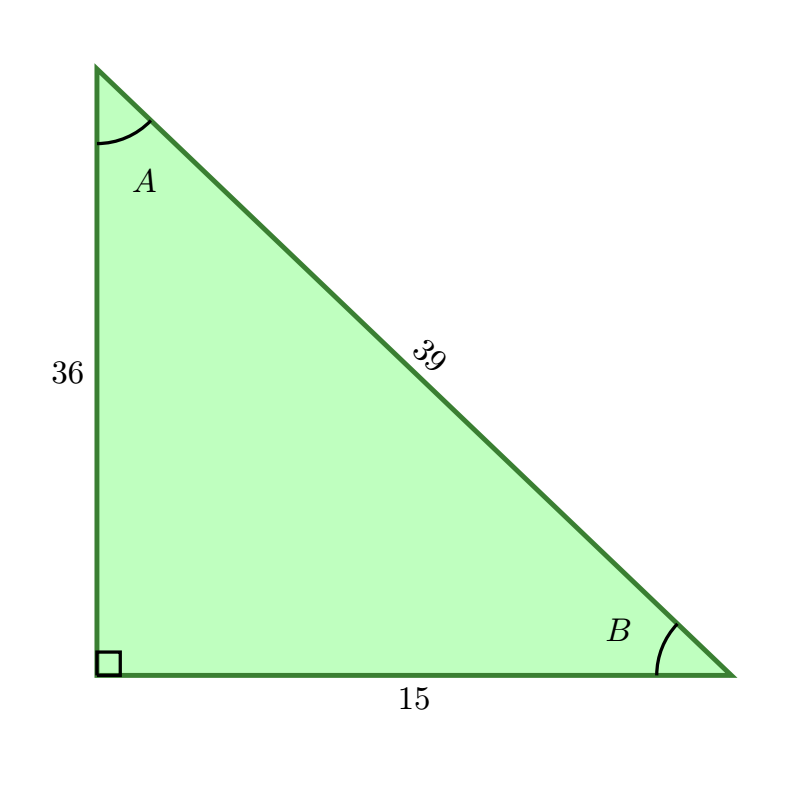
\includegraphics[width=0.9\linewidth]{mex_0086.png} \\ cos($A$)=\fillin[$0.92$][0cm]}
            \end{parts}
        \end{multicols}
    }

    \subsection*{Encontrando lados}

    \ejemplosboxed[{Usando la función trigonométrica correcta, encuentra el valor de los lados $x$, para cada uno de los siguientes ejercicios:

                \begin{multicols}{2}
                    \begin{parts}
                        \part  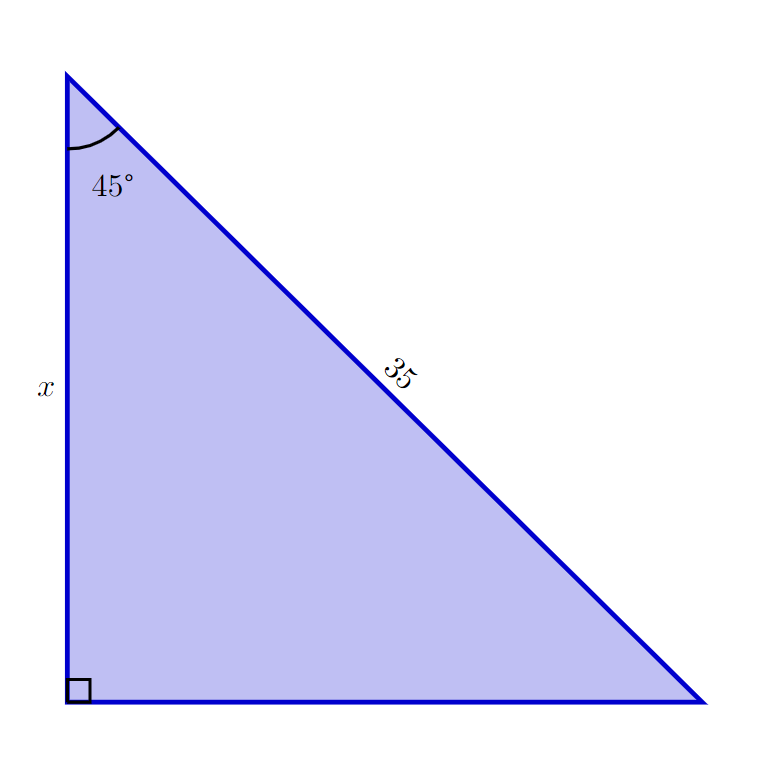
\includegraphics[width=0.75\linewidth]{mex_0091.png} \\ $x=$\fillin[$37.08$][0cm]
                        \part 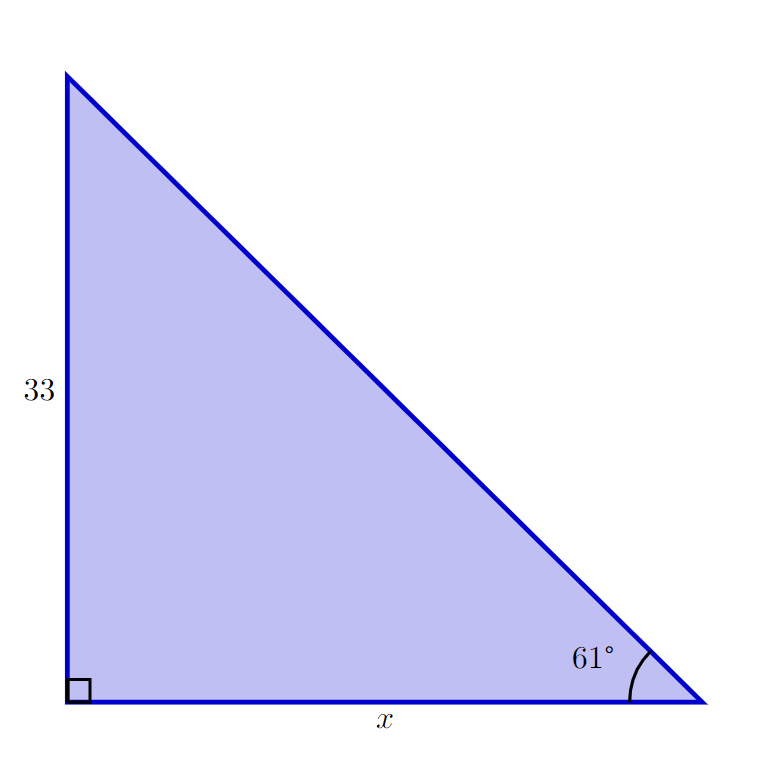
\includegraphics[width=0.75\linewidth]{mex_0092.png}  \\ $x=$\fillin[$24.84$][0cm]
                    \end{parts}
                \end{multicols}
            }]

    \questionboxed[3]{Usando la función trigonométrica correcta, encuentra el valor de los lados $x$, para cada uno de los siguientes ejercicios:

        \begin{multicols}{3}
            \begin{parts}
                \part  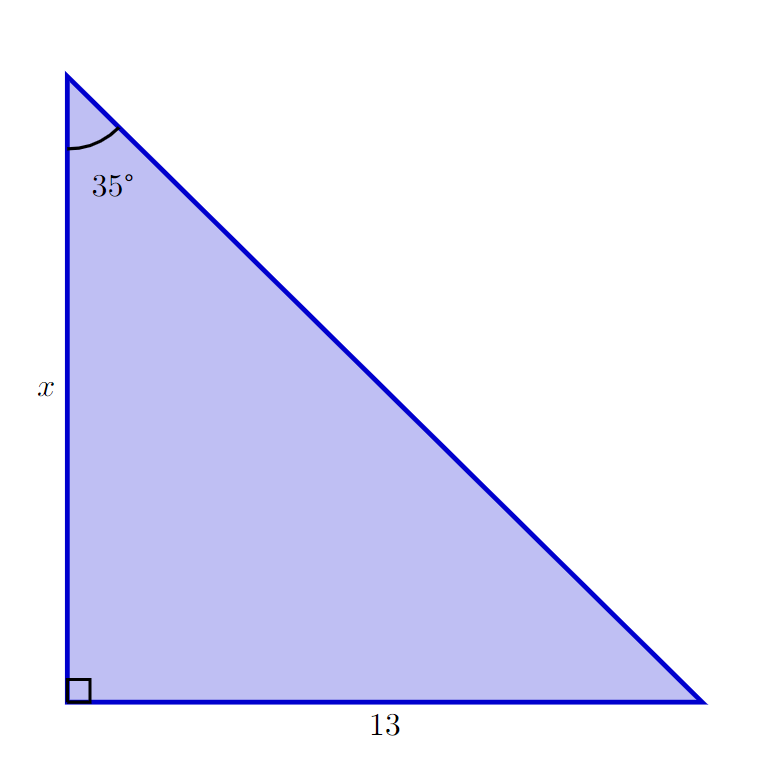
\includegraphics[width=0.9\linewidth]{mex_0093.png}  \\ $x=$\fillin[$18.56$][0cm]
                \part 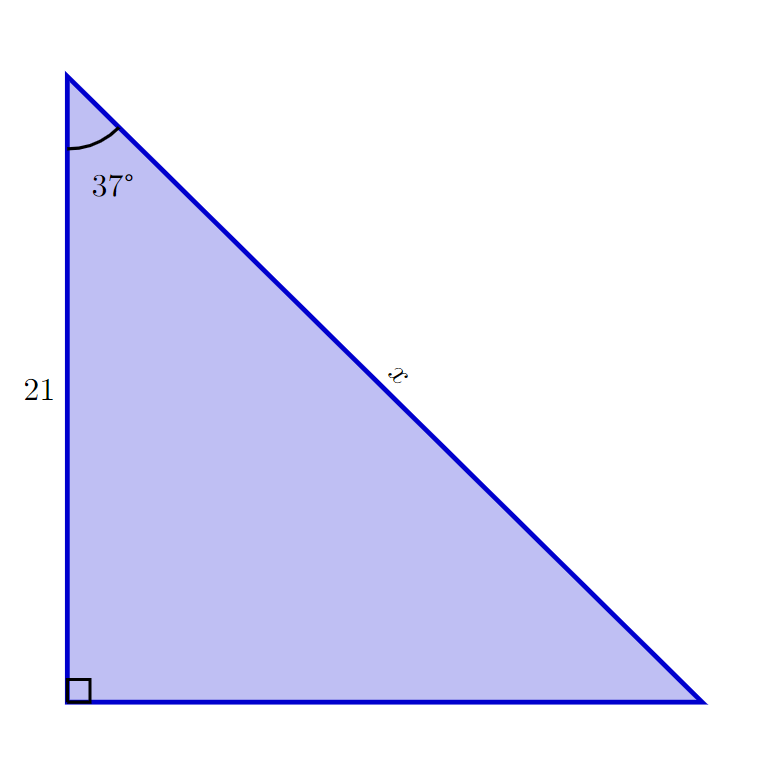
\includegraphics[width=0.9\linewidth]{mex_0094.png}   \\ $x=$\fillin[$26.29$][0cm]
                \part  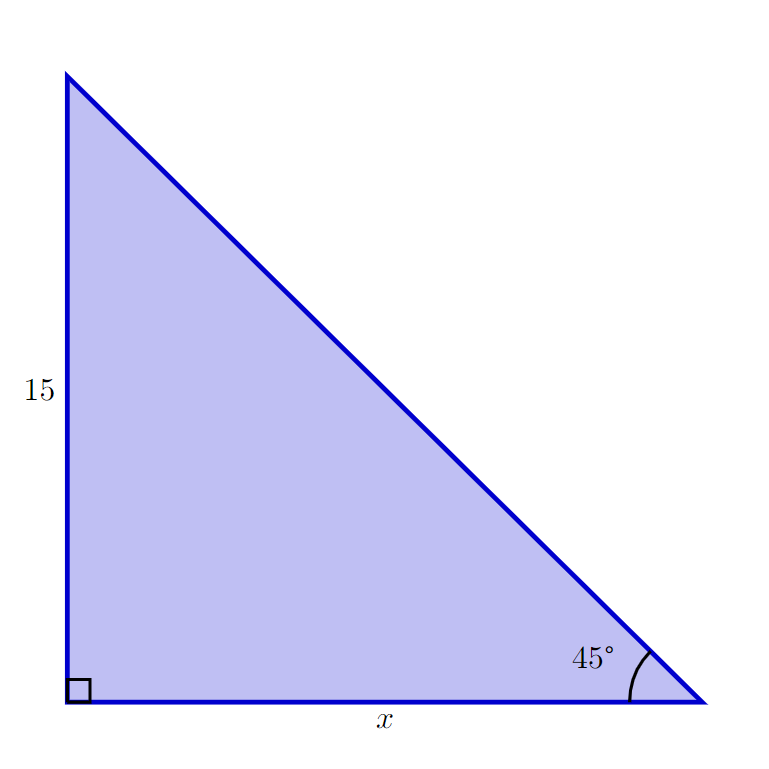
\includegraphics[width=0.9\linewidth]{mex_0095.png}  \\ $x=$\fillin[$18.29$][0cm]
            \end{parts}
        \end{multicols}
    }

    \subsection*{Encontrando ángulos}

    \ejemplosboxed[{Usando la función trigonométrica correcta, encuentra el valor de los ángulos $x$, para cada uno de los siguientes ejercicios:

                \begin{multicols}{2}
                    \begin{parts}
                        \part  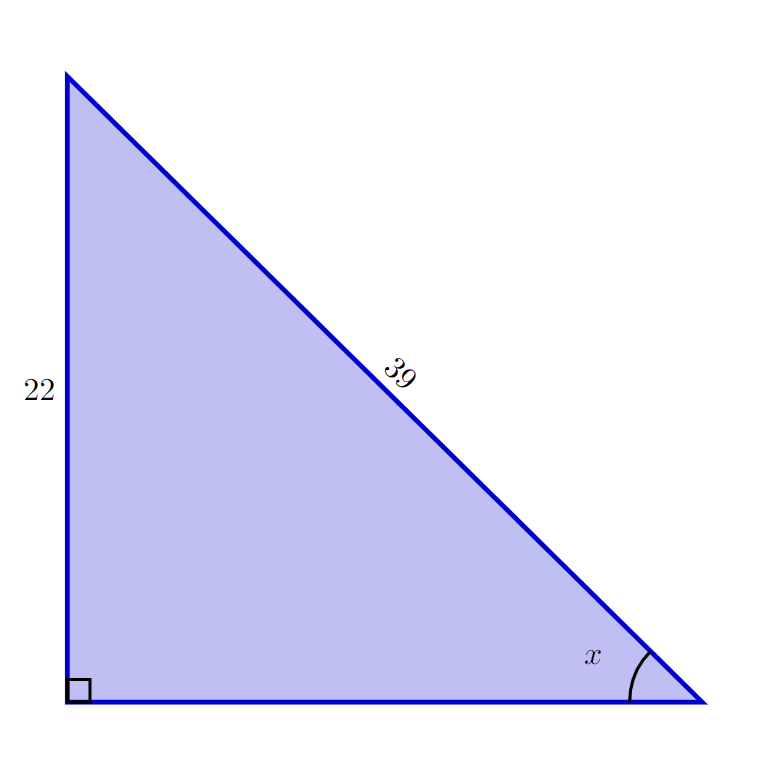
\includegraphics[width=0.75\linewidth]{mex_0096.png} \\ $x=$\fillin[$34.33$][0cm]
                        \part 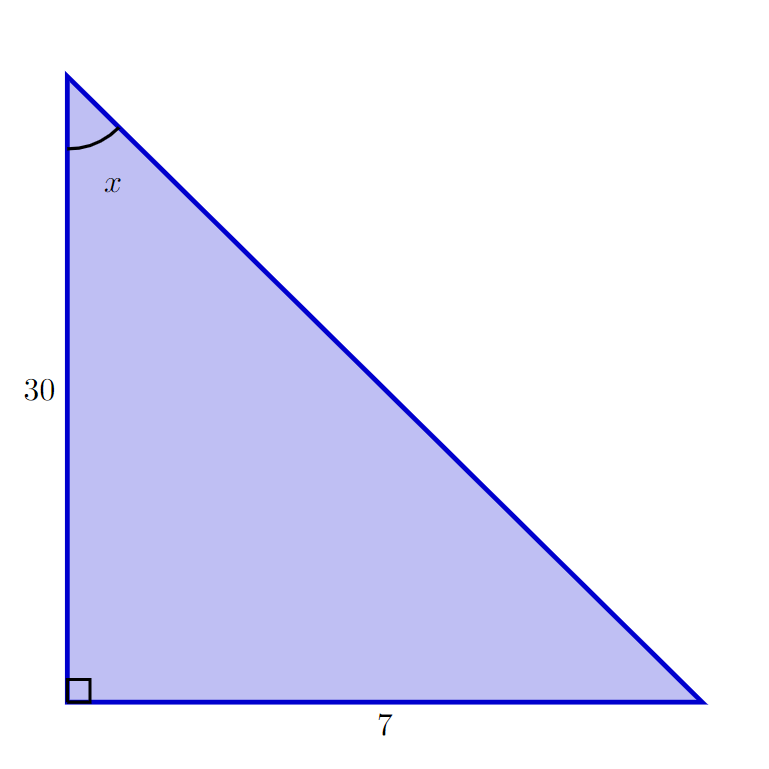
\includegraphics[width=0.75\linewidth]{mex_0097.png}  \\ $x=$\fillin[$13.13$][0cm]
                    \end{parts}
                \end{multicols}
            }]

    \questionboxed[6]{sando la función trigonométrica correcta, encuentra el valor de los ángulos $x$, para cada uno de los siguientes ejercicios:

        \begin{multicols}{3}
            \begin{parts}
                \part  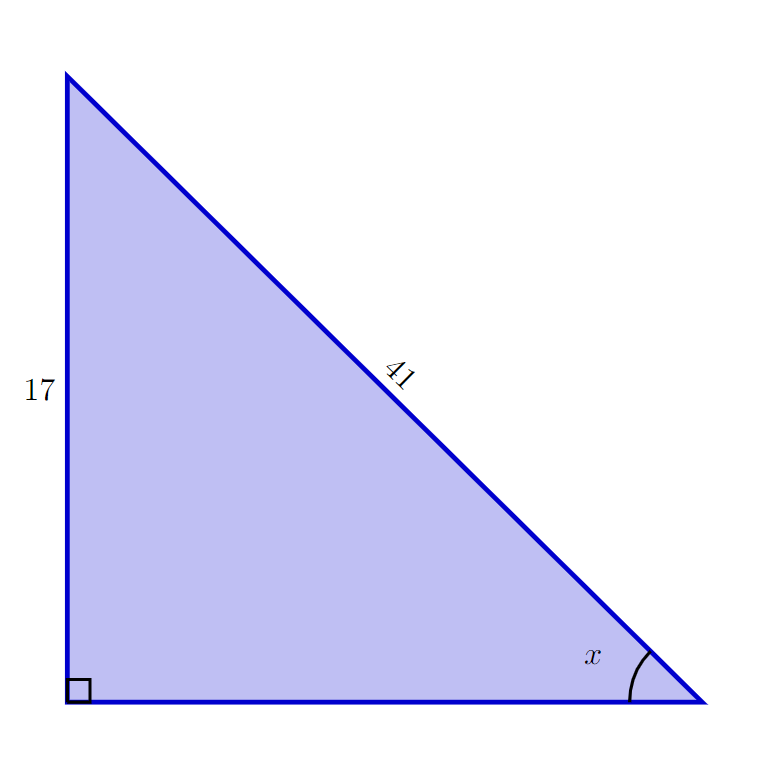
\includegraphics[width=0.9\linewidth]{mex_0098.png}  \\ $x=$\fillin[$24.49$][0cm]
                \part 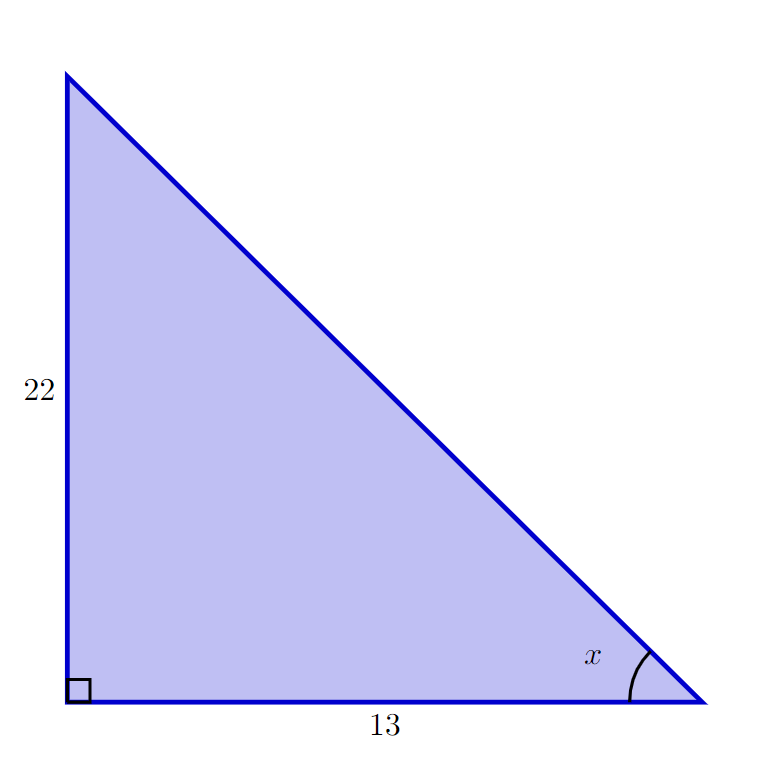
\includegraphics[width=0.9\linewidth]{mex_0099.png}   \\ $x=$\fillin[$59.42$][0cm]
                \part  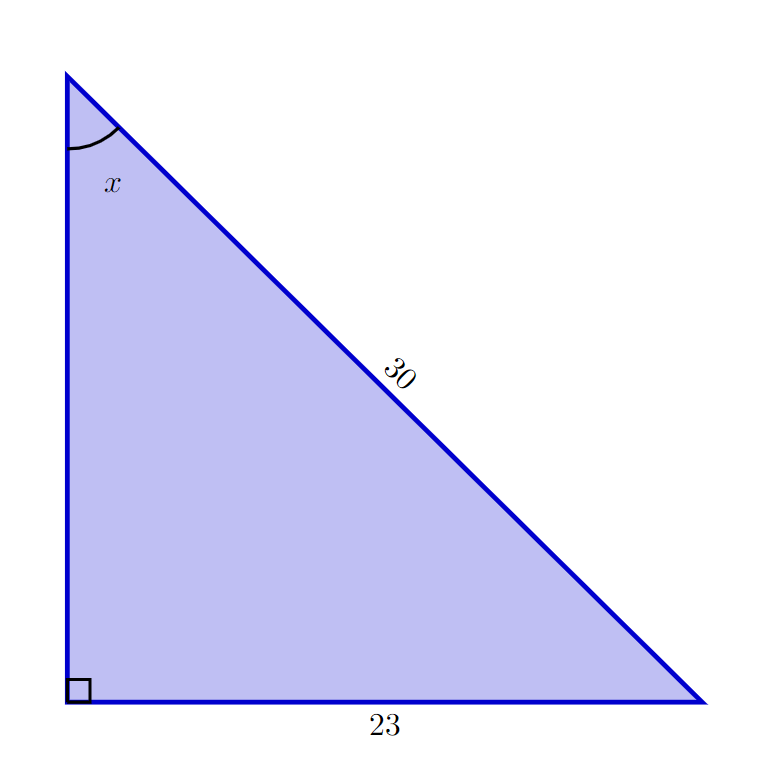
\includegraphics[width=0.9\linewidth]{mex_0100.png}  \\ $x=$\fillin[$50.05$][0cm]
            \end{parts}
        \end{multicols}
    }

    \subsection*{Resolución de problemas}

    \ejemplosboxed[{Resuelve los siguientes problemas:

                \begin{multicols}{2}
                    \begin{parts}
                        \part  El piloto de un avión debe aproximarse a la pista de aterrizaje con un ángulo de 7° con respecto a la horizontal. Si vuela a una altura de 8,000 metros, ¿a qué distancia de la pista debe iniciar su descenso?

                        \begin{solutionbox}{2cm}
                            65154.77
                        \end{solutionbox}

                        \part El sonar de un barco de salvamiento localiza los restos de un naufragio en un ángulo de depresión de 40°. Un buzo es bajado 40 metros hasta el fondo del mar, ¿cuánto necesita avanzar el buzo por el fondo para encontrar los restos del naufragio?

                        \begin{solutionbox}{2cm}
                            47.67
                        \end{solutionbox}
                    \end{parts}
                \end{multicols}
            }]

    \questionboxed[6]{Resuelve los siguientes problemas:
        % \begin{multicols}{3}
        \begin{parts}
            \part Cuando el sol se encuentra a 20° sobre el horizonte, ¿cuánto medirá la sombra proyectada por un edificio de 50 m de altura?

            \begin{solutionbox}{2cm}
                137.37
            \end{solutionbox}

            \part Una escalera de extensión de 7.62 metros recargada contra un edificio forma un ángulo de 70° con el suelo. ¿A qué altura del edificio llega la escalera?

            \begin{solutionbox}{2cm}
                7.16
            \end{solutionbox}

            \part  La diagonal de un rectángulo mide 8.25 cm y el menor de sus lados mide 3.14 cm. Calcula el ángulo formado por la diagonal y el lado mayor del rectángulo.

            \begin{solutionbox}{2cm}
                22.33
            \end{solutionbox}
        \end{parts}
        % \end{multicols}
    }
\end{questions}
\end{document}